% !Mode:: "TeX:UTF-8"
\chapter{基于多尺度特征融合的点云几何特征检测}
\label{chap:necdnet}

\section{引言}
% 分析边缘与角点特征的模糊性及检测难点。
三维点云几何特征检测（如边缘和角点的提取）是三维视觉领域的关键环节，在模型重建、物体识别及机器人抓取规划中具有不可替代的作用。传统的分析方法主要依赖于局部几何描述符（如曲率、法向量偏差等）并结合人工设置的阈值。然而，由于点云数据存在噪声、密度不均以及边缘及角点定义模糊等问题，传统方法往往难以兼顾检测精度与鲁棒性~\cite{}。

为了解决边缘与角点特征在微小尺度下难以区分的问题，本章提出了一种名为 NECDNet（Neural Edge and Corner Detection Network）的深度学习架构。该方法通过融合统计特征描述符与轻量级神经网络，利用多尺度邻域分析来捕捉点云局部的空间分布和法向量变化特征，从而实现对面点（Face）、边缘点（Edge）和角点（Corner）的高精度同步分类。

图~\ref{fig:necdnet_framework}展示了所提 NECDNet 的工作流程，NECDNet 由两个主要部分组成：多尺度局部特征矩阵计算和基于神经网络的分类器。流程的输入是一个非结构化点云，输出的是一个三类点云，包含面点、边缘点和角点。在多尺度特征计算阶段，我们针对每个查询点构建了包含四个不同尺度邻域的特征矩阵，每个尺度下计算六种解析特征：曲率、投影距离、均值中心距离、法向角差、法向分布和投影法向模。最终形成一个 4$\times$6 的多尺度特征矩阵，作为神经网络的输入。在分类器阶段，我们基于多层感知机（MLP）设计了一个层次化网络结构，通过逐层融合多尺度特征，学习从特征矩阵到几何类别的映射关系。输出三类几何特征的概率得分，从而实现面、边缘和角点的同步检测。

图中左上为输入的点云数据，每次选择一个查询点（红色）及其邻域（绿色）。其中不同的$k$值表示不同尺度的邻域大小（黄色点的数量）。通过计算各尺度下的六维特征，形成多尺度特征矩阵并输入神经网络进行分类。最终输出查询点所属的几何类别（面、边缘或角点）。通过循环查询各个点，完成整个点云的几何特征检测任务，最后输出检测结果（左下）。


\begin{figure}[!htbp]
    \centering
    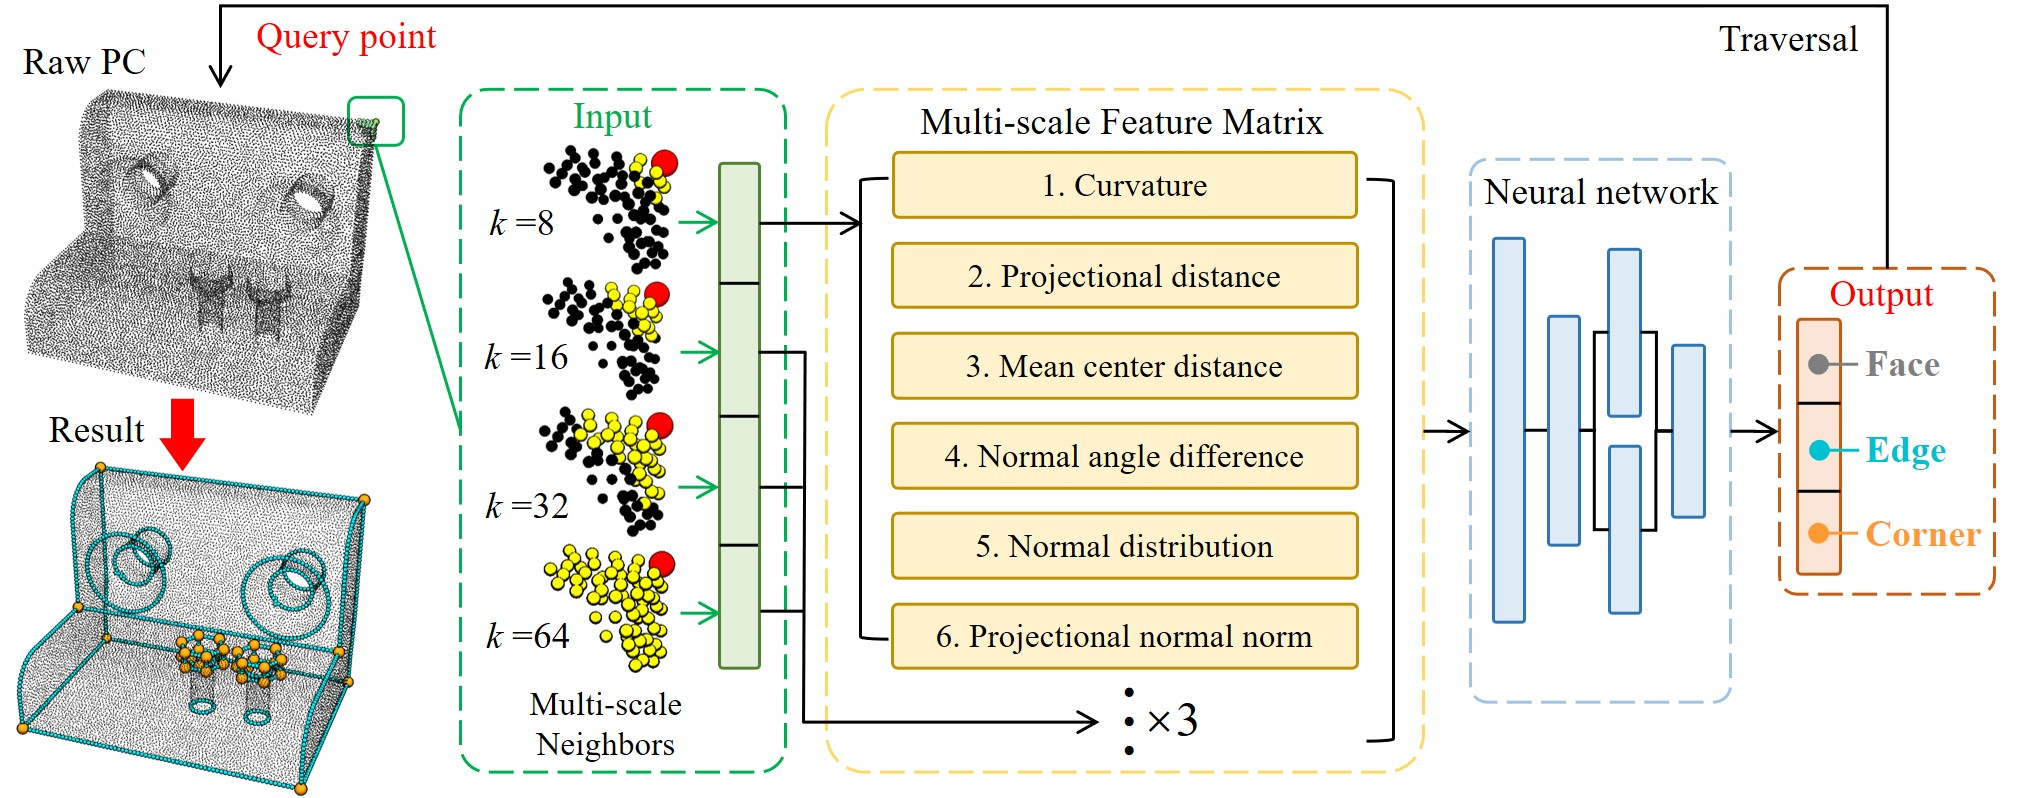
\includegraphics[width=1.0\textwidth]{NECDNet/workflow.jpg}
    \bicaption{NECDNet 网络架构及工作流程示意图。}{NECDNet network architecture and workflow diagram.}
    \label{fig:necdnet_framework}
\end{figure}


\section{多尺度局部特征提取与计算}
多尺度表示的是针对每个查询点，选择不同数量的邻域点以构建多层次的局部几何描述。由于点云捕获时的视角、距离及分辨率等因素影响，单一尺度往往难以全面反映局部几何结构的信息。
通过分析不同尺度下的点云分布特征，可以更全面地捕捉局部几何结构，从而提升边缘和角点的区分能力~\cite{}。适用的尺度取决于多个因素：物体大小、形状复杂度、点云密度、观察尺度等。为了使训练得到的模型能泛化处理未知物体的情况，本文为输入点云中的每个查询点在多尺度邻域内计算多个特征，并在~\ref{cha:xx}进行了消融实验确保各个尺度选择的合理性。

\subsection{多尺度邻域构建}
% 解释 k 近邻搜索与多尺度选择策略。
本文采用基于距离度量的 $k$ 近邻（k-Nearest Neighbors, k-NN）为每个查询点构建多尺度邻域，并以此生成多尺度特征输入网络进行学习~\cite{}。k-NN 是一种基于距离度量的邻域选择方法，通过计算查询点与其他点之间的欧氏距离，选取距离最近的 $k$ 个点作为邻域。与固定半径（radius-based）邻域相比，k-NN 对点云非均匀采样与稀疏区域更加稳健：在稠密区不会过采样、在稀疏区不会因样本不足而破坏特征稳定性。对于非结构化的点云，其只包含点的三维坐标信息，k-NN 方法能够有效适应点云的稀疏性和不均匀分布特性。

为提升检索效率，给定一个非结构化点云 $\mathcal{P}^\text{c} = \{\mathbf{p}_i^\text{c} \mid i = 1, \dots, n\}$，我们在三维坐标空间上构建 KD-树（K-Dimensional Tree）索引~\cite{}。KD-树通过在各坐标轴上递归划分点集，使每个节点对应一个超矩形子空间，从而形成近似平衡的二叉树。查询时，先依据查询点坐标自顶向下定位至叶节点，再在回溯过程中检查可能包含更近邻点的分支，并维护容量为 $k$ 的候选集合以持续更新最近邻。相比于暴力检索的 $O(n)$ 复杂度，KD-树可将单次最近邻查询的平均复杂度降至 $O(\log n)$ ，显著提升大规模点云处理的效率。

基于上述索引结构，对每个查询点 $\mathbf{p}_i^\text{c}$，我们通过 k-NN 方法在点云中搜索其 $k$ 个最近邻点，形成邻域集合 $\mathcal{Q}_i^\text{c} = \{\mathbf{p}_{i,j}^\text{c} \mid j = 1, \dots, k\}$。通过调节 $k$ 的大小即可改变邻域的空间尺度：较小的 $k$ 更敏感于细粒度几何细节（如尖锐小角、细薄边），较大的 $k$ 则能稳健表征更大范围的局部结构。为兼顾不同尺度的几何信息，我们针对多个 $k$ 值为同一查询点构建多组邻域，形成多尺度邻域表示。

具体而言，对由给定 $k$ 值确定的局部区域 $\mathcal{Q}_i^\text{c}$ 计算六个解析特征，得到 6 维特征向量 $\mathbf{x}_i^\text{c}$。当为同一查询点在多个 $k$ 值下重复上述过程，即可获得对应的 $\mathbf{x}_{i,k}^\text{c}$。将这些特征按尺度汇集，构成用于后续网络学习的多尺度特征矩阵，如公式~(\ref{eq:X_i}) 所示：
\begin{equation}
    \mathbf{X}_{i}^\text{c}=\begin{bmatrix}
    \mathbf{x}_{i, k_{1}}^\text{c} \\
    \mathbf{x}_{i, k_{2}}^\text{c} \\
    \vdots \\
    \mathbf{x}_{i, k_{m}}^\text{c}
    \end{bmatrix}
    \label{eq:X_i}
\end{equation}

其中，$k_1, k_2, \ldots, k_m$ 表示所选择的不同邻域尺度，$m$ 为尺度数量。多尺度特征矩阵中的尺度数$m$ 和尺度大小 $k$ 直接影响神经网络的学习结果。具体来说，$k$ 影响结果对点云不同稀疏度的适用性，而 $m$ 影响网络学习数据的维度。选择合适的尺度尺寸和数量可以优化检测精度。因此，在第\ref{}章中，本文对邻近尺度选择进行了消融实验以确定参数，并选择了 $k$ 的四个值：8、16、32和64进行特征计算。

\subsection{局部特征描述符设计}
% 详细介绍位置特征（曲率、投影距离、均值中心距离）和法向量特征（法向角差、法向分布、投影法向模）。

在构建多尺度邻域的基础上，本文进一步设计了一套包含六个维度的局部几何特征描述符，旨在精确捕捉查询点及其邻域在不同空间尺度下的结构属性。这六种特征可归纳为基于位置的几何特征（Position-based Features）与基于法向量方向的特征（Normal-based Features）两大类。
基于位置的特征主要通过分析邻域点的空间分布规律来描述局部形状，而基于法向量的特征则通过分析表面方向的连续性与一致性，提供关于几何边缘与尖锐角点的关键判别信息。这种多维特征的结合，增强了模型在面对复杂、模糊边界时的区分能力。消融实验中对特征计算中涉及的所有描述符进行了评估，说明了该选择的有效性。

\subsubsection{邻域归一化预处理}
% 解释邻域中心化与尺度归一化的步骤与目的。

为了消除点云绝对坐标、平移以及尺度差异对特征计算的影响，在提取特征前，本文首先对邻域 $\mathcal{Q}_i^\text{c}$ 进行归一化处理。该过程基于主成分分析（Principal Component Analysis, PCA）思想，计算邻域点的协方差矩阵 $\mathbf{K}_i = \mathrm{cov}(\mathcal{Q}_i^\text{c})$，并对其进行奇异值分解（Singular Value Decomposition, SVD），如公式(\ref{eq:svd_Ki}) 所示。
\begin{equation}
\mathbf{K}_i = \mathbf{U}_i \boldsymbol{\Sigma}_i \mathbf{V}_i^T
\label{eq:svd_Ki}
\end{equation}

其中，$\mathbf{U}_i$ 和 $\mathbf{V}_i$ 分别为左奇异向量矩阵和右奇异向量矩阵，$\boldsymbol{\Sigma}_i$ 为对角奇异值矩阵。通过该分解，我们能够获得邻域点在主方向上的分布特性。具体而言，通过对角矩阵 $\boldsymbol{\Sigma}_i$ 提取奇异向量 $\boldsymbol{\sigma}_i = (\sigma_{i,1}, \sigma_{i,2}, \sigma_{i,3})$ ，其中的奇异值计为降序排列。右奇异向量矩阵 $\mathbf{V}_i$ 的列向量对应于邻域点在三个主方向上的投影轴。不同的奇异值反映了邻域点在各主方向上的扩展程度。奇异值较小的方向点云分布较为集中，反之则较为分散。
通过上述分解结果，可以对邻域点进行去中心化与尺度归一化处理。具体而言，首先计算邻域点的质心 $\bar{\mathbf{p}}_{i,j}^\text{c}$ ，如公式(\ref{eq:center_Qi})所示。其中$|\mathcal{Q}_i^\text{c}|$ 表示邻域点的数量。
\begin{equation}
    \bar{\mathbf{p}}_{i,j}^\text{c} = \frac{1}{|\mathcal{Q}_i^\text{c}|} \sum_{j=1}^{k} \mathbf{p}_{i,j}^\text{c}
    \label{eq:center_Qi}
\end{equation}22

随后，将所有邻域点坐标减去质心实现去中心化，并利用奇异值 $\sigma_{i,1}$ 和 $\sigma_{i,2}$ 对去中心化后的邻域点进行尺度缩放，确保各个方向上的分布具有统一的量纲，如公式(\ref{eq:norm_Qi})所示。最终，得到归一化后的邻域 $\hat{\mathcal{Q}}_i^\text{c}$，为后续特征计算提供了标准化的输入。归一化邻域后的查询点坐标记为 $\hat{\mathbf{p}}_i^\text{c}$，邻域中的点坐标记为 $\hat{\mathbf{p}}_{i,j}^\text{c}$。
\begin{equation}
    \hat{\mathcal{Q}}_i^\text{c} = \left\{ \frac{2}{\sqrt{\sigma_{i,1}} + 
    \sqrt{\sigma_{i,2}}} \left( \mathbf{p}_{i,j}^\text{c} - \bar{\mathbf{p}}_{i,j}^\text{c} \right) \mid 
    \mathbf{p}_{i,j}^\text{c}\in \mathcal{Q}_i^\text{c} \right\}
    \label{eq:norm_Qi}
\end{equation}

\subsubsection{点云法向量估计}
\label{sec:normal_estimatation}
法向量是描述点云局部表面方位的重要几何属性，也是计算后续方向特征的基础。本文采用基于局部平面拟合的方法估计查询点的法向量。
从公式 (\ref{eq:svd_Ki}) 的奇异值分解结果中可知，奇异值 $\sigma_{i,1}, \sigma_{i,2}, \sigma_{i,3}$ 对应的右奇异向量（即矩阵 $\mathbf{V}_i$ 的列向量）构成了邻域内点集分布的正交主轴。由于奇异值按降序排列，最小奇异值 $\sigma_{i,3}$ 对应的奇异向量 $\mathbf{v}_{i,3}$ 指向了邻域内点集分布方差最小的方向。在几何意义上，该方向与局部最小二乘拟合平面的法向重合。因此，查询点的法向量 $\mathbf{n}_i^\text{c}$ 可直接取为归一化后的右奇异向量 $\mathbf{v}_{i,3}$ 。

然而，仅通过 PCA 获得的法向量存在 $180^\circ$ 的方向模糊性（即法向量可能指向物体内侧或外侧）。为了确保在计算后续法向量夹角差异等特征时的数值一致性，必须对法向量进行定向处理。
在处理具有闭合表面的物体时，通常利用视点方向或邻域一致性进行约束。本文采用最小生成树（Minimum Spanning Tree, MST）算法在点云图中传播法向量方向，以实现全局的方向一致化~\cite{}。具体而言，将点云视为图结构，以点间距离为边权构建图，从初始点开始，通过遍历图确保相邻点的法向量满足内积大于零的约束，实现对点云中各点法向量的方向一致化。

\subsubsection{曲率（ $\kappa_i$ ）}
% 差一张插图
首先计算基于位置的几何特征，表征邻域内点的几何分布特性。曲率 $\kappa_i$ 是几何物体偏离平面程度的度量。在本文中，查询点邻域的曲率可以根据上述得到的奇异值进行计算，用于表征局部表面的平坦程度。具体而言，曲率定义为最大奇异值与三维奇异值之和的比值，如公式(\ref{eq:curvature})所示。
\begin{equation}
    \kappa_i = \frac{\sigma_{i,3}}{\sigma_{i,1} + \sigma_{i,2} + \sigma_{i,3}}
    \label{eq:curvature}
\end{equation}

当查询点位于平坦表面时，$\sigma_{i,3}$ 较小，曲率值接近于零；而当查询点位于尖锐边缘或角点时，$\sigma_{i,3}$ 较大，曲率值相应增大。因此，曲率特征有助于区分面点与边缘、角点。

\subsubsection{投影距离均值（ $\bar{d_i}$ ）}
% 差一张插图
投影距离均值 $\bar{d_i}$ 用于刻画查询点邻域内点相对于该点法向平面的空间分布，其大小反映了局部几何结构的突变程度。具体地，对于任一查询点 $\hat{\mathbf{p}}_i^\text{c}$，结合其法向量 $\mathbf{n}_i^\text{c}$ 可定义通过该点的投影平面。邻域内所有点 $\hat{\mathbf{p}}_{i,j}^\text{c}$ 到该投影平面的距离均值即为 $\bar{d}_i$，计算公式如(\ref{eq:projection_distance})所示。
\begin{equation}
    \bar{d}_i = \frac{1}{|\hat{\mathcal{Q}}_i^\text{c}|} \sum_{\hat{\mathbf{p}}_{i,j}^\text{c} \in \hat{\mathcal{Q}}_i^\text{c}} \left| (\hat{\mathbf{p}}_{i,j}^\text{c} - \hat{\mathbf{p}}_i^\text{c}) \cdot \mathbf{n}_i^\text{c} \right|
    \label{eq:projection_distance}
\end{equation}

图~\ref{}展示了该距离度量的几何意义。其反映了邻域点在查询点法向方向上的分布特性：当邻域点主要分布在查询点法向平面附近时，投影距离较小，表明局部几何结构较为平滑；而当邻域点在法向方向上分布较为分散时，投影距离增大，通常对应于边缘或角点区域。

\subsubsection{中心偏离比（ $r_i$ ）}
中心偏离比 $r_i$ 是量化查询点在其局部邻域内的相对空间位置的度量，其能够衡量查询点相对于其邻域质心的偏移程度。具体而言，首先计算邻域点的质心，由于此时的邻域 $\hat{\mathcal{Q}}_i^\text{c}$ 已经进行了去中心化及归一化处理，因此邻域质心即为原点。之后计算查询点到质心的距离 $\| \hat{\mathbf{p}}_i^\text{c} \|$ 与邻域内各点到质心距离 $\| \hat{\mathbf{p}}_{i,j}^\text{c}\|$ 的最小值之比，得到中心距离均值比 $r_i$，计算公式如(\ref{eq:mean_center_distance})所示，由于该特征为比值，当分母较小时产生的结果不受此前归一化邻域的影响。故针对特征 $r_i$，本文选用 Sigmoid 函数对其进行标准化处理，以减小数值分布的变化范围。
\begin{equation}
    r_i = \operatorname{Sigmoid}\left(\frac{\| \hat{\mathbf{p}}_i^\text{c} \|}{\min_{\hat{\mathbf{p}}_{i,j}^\text{c} \in \hat{\mathcal{Q}}_i^\text{c}} \| \hat{\mathbf{p}}_{i,j}^\text{c}\|}\right)
    \label{eq:mean_center_distance}
\end{equation}

其中 $\operatorname{Sigmoid}$ 表示 Sigmoid 函数，$\| \cdot \|$ 表示欧氏距离，$\min$ 运算符用于获取邻域点中距离质心最近的点的距离，式中省略了减去质心零向量的表示。中心偏离比 $r_i$ 反映了查询点在邻域内的相对位置关系：当查询点位于邻域质心附近时，$r_i$ 值较小，表明该点可能位于平坦区域；而当查询点远离邻域质心时，$r_i$ 值增大，通常对应于边缘或角点区域。因此，中心偏离比有助于区分不同几何特征。

\subsubsection{法向量角度差（$\mu_{\theta,i}$）}
以此特征描述符开始，后续的三个描述符是基于法向量方向的特征，旨在捕捉表面方向的突变信息。法向角度差 $\mu_{\theta,i}$ 衡量查询点法向量与其邻域内各点法向量之间夹角的平均值，反映了局部表面方向的一致性。具体而言，首先根据章节\ref{sec:normal_estimatation}中的方法估计邻域内每个点的单位法向量 $\mathbf{n}_{i,j}^\text{c}$，组合为 $\mathcal{N}_i^\text{c}$。随后，计算查询点法向量 $\mathbf{n}_i^\text{c}$ 与邻域内各点法向量之间的夹角 $\theta_{i, j}$ ，计算公式如(\ref{eq:normal_angle})。最后并求各个夹角的平均值，求解公式如(\ref{eq:normal_angle_difference})所示。
\begin{equation}
    \theta_{i,j} = \arccos \left( \mathbf{n}_i^\text{c} \cdot \mathbf{n}_{i,j}^\text{c} \right)
    \label{eq:normal_angle}
\end{equation}
\begin{equation}
    \mu_{\theta,i} = \frac{1}{|\mathcal{N}_i^\text{c}|} \sum_{j=1}^{|\mathcal{N}_i^\text{c}|} \theta_{i,j}
    \label{eq:normal_angle_difference}
\end{equation}

其中，$\arccos$ 表示反余弦函数。法向角度差 $\mu_{\theta,i}$ 反映了邻域内法向量的方向变化程度：当邻域内法向量与查询点法向量高度一致时，$\mu_{\theta,i}$ 值较小，表明局部表面较为平滑；而当邻域内法向量与查询点法向量差异较大时，$\mu_{\theta,i}$ 值增大，通常对应于边缘或角点区域。

此外，除了用法向量夹角来表示方向变化外，还可以直接使用法向量的数值之差来表示方向变化。具体而言，计算查询点法向量与邻域内各点法向量的差值，并求其平均值，得到法向量数值差 $\bar{\Delta \mathbf{n}}_i$，计算公式如(\ref{eq:normal_value_difference})所示。相较与法向量角度差 $\mu_{\theta,i}$，法向量数值差 $\bar{\Delta \mathbf{n}}_i$ 直接采用原始法向量数据进行统计计算，后续消融实验中会讨论两者的效果差异。
\begin{equation}
    \bar{\Delta \mathbf{n}}_i = \frac{1}{|\mathcal{N}_i^\text{c}|} \sum_{\mathbf{n}_{i,j}^\text{c} \in \mathcal{N}_i^\text{c}} ( \mathbf{n}_i^\text{c} - \mathbf{n}_{i,j}^\text{c} )
    \label{eq:normal_value_difference}
\end{equation}

\subsubsection{法向量分布方差（ $\sigma^2_{\theta,i}$ ）}
法向量分布方差 $\sigma^2_{\theta,i}$ 用于量化邻域内法向量夹角的变化剧烈程度，反映了局部表面方向的稳定性。具体而言，基于前述计算的法向角度差 $\mu_{\theta,i}$，计算邻域内各点法向量与查询点法向量夹角的方差，求解公式如(\ref{eq:normal_distribution_variance})所示。
\begin{equation}
    \sigma^2_{\theta,i} = \frac{1}{|\mathcal{N}_i^\text{c}|} \sum_{j=1}^{|\mathcal{N}_i^\text{c}|} (\theta_{i,j} - \mu_{\theta,i})^2
    \label{eq:normal_distribution_variance}
\end{equation}

法向量分布方差 $\sigma^2_{\theta,i}$ 反映了邻域内法向量变化的剧烈程度：当邻域内法向量夹角较为集中时，$\sigma^2_{\theta,i}$ 值较小，表明局部表面方向较为稳定；而当邻域内法向量夹角分布较为分散时，$\sigma^2_{\theta,i}$ 值增大，通常对应于边缘或角点区域，而角点区域的分散程度更为显著。

\subsubsection{法线投影距离均值（ $\bar{\text{proj}_i}$ ）}
法线投影距离均值 $\bar{\text{proj}_i}$ 用于量化邻域点法向量在查询点法向上的投影强度，反映了表面法向的对齐程度。具体而言，计算邻域内每个点法向量 $\mathbf{n}_{i,j}^\text{c}$ 在查询点法向 $\mathbf{n}_i^\text{c}$ 上的投影长度，并求其平均值，计算公式如(\ref{eq:projectional_normal_norm})所示。
\begin{equation}
    \bar{\text{proj}_i} = \frac{1}{|\mathcal{N}_i^\text{c}|} \sum_{\mathbf{n}_{i,j}^\text{c} \in \mathcal{N}_i^\text{c}} \left| \mathbf{n}_{i,j}^\text{c} \cdot \mathbf{n}_i^\text{c} \right|
    \label{eq:projectional_normal_norm}
\end{equation}

由于各点的法向量均为单位向量，法线投影距离均值 $\bar{\text{proj}_i}$ 可以反映邻域内法向量与查询点法向量的对齐程度：$\bar{\text{proj}_i}$ 值较大，表明局部表面方向较为统一；而当邻域内法向量与查询点法向量差异较大时，$\bar{\text{proj}_i}$ 值减小，通常对应于边缘或角点区域。

\subsection{局部特征描述符数值可视化分析}
% 展示不同特征在区分面、边、角时的分布差异。
通过上述计算的局部特征描述符，本文最终选择了其中六个组成特征描述向量，并用于后续的特征融合和分类任务。最后得到的特征向量如公式(\ref{eq:feature_vector})所示。六个特征均为标量，组成的特征向量维度为 6，包含了点云的位置分布特性和法向量变化信息，能够有效表征点云局部的几何结构属性。
\begin{equation}
    \mathbf{x}_i^\text{c} = \left( \kappa_i, \bar{d}_i, r_i, \mu_{\theta,i}, \sigma^2_{\theta,i}, \bar{\text{proj}_i} \right)
    \label{eq:feature_vector}
\end{equation}

图~\ref{fig:feature_distribution} 展示了多尺度几何特征在点云三类特征（面、边缘、角点）中的分布表现，直观体现了所选六维特征向量对于区分不同几何类别的有效性。
其中图(a)对单个物体点云的六个特征进行了空间分布可视化。每个子图分别显示了特征描述符 $\kappa_i$（曲率）、$\bar{d}_i$（投影距离均值）、$r_i$（中心偏离比）、$\mu_{\theta,i}$（法向量角度差）、$\sigma^2_{\theta,i}$（法向量分布方差）、$\bar{\text{proj}_i}$（法向投影距离均值）在点云空间上的数值分布情况。颜色表示数值大小，采用从蓝色（低值）到红色（高值）的渐变色带。根据上一小节对各特征的定义，可以观察到：除了特征$\bar{\text{proj}_i}$外，其他五个特征在面、边缘和角点区域均表现出从低到高的数值变化趋势（蓝色到红色）。而特征$\bar{\text{proj}_i}$ 则呈现出相反的趋势，在面区域数值较高（红色），而在边缘和角点区域数值降低（橙黄色）。各个特征在不同的几何结构上有着明显的区别。

图(b)部分给出了在我们构建的数据集ABC-Corner中1000个点云样本的六个特征在三类标签下的数值分布，数据集的描述及构建过程请见章节(\ref{sec:dataset})。纵轴为点云ID，横轴为特征值，颜色标记类别：蓝色为面、黄色为边缘、红色为角点。统计结果显示，在面、边缘、角点三类之间，所有特征分布具有明显的界限。
以曲率和法向分布为例，角点（红色）主要集中在中高值段，面点则聚集于低值，边缘点分布于中间区域。其他如投影距离、均值中心距离等特征也展现出对类别的良好区分能力。

虽然可以观察到直接使用这些特征描述符就能进行一定程度上的几何特征区分。然而，直接使用这些特征进行检测类似于分析方法，需要参数调整并且可能无法保证稳健的结果。为了解决这个问题，本文利用神经网络从计算的特征矩阵中学习。这种方法使能够结合分析方法和基于学习的检测技术的优势，实现精准的自分类。
\begin{figure}
    \centering
    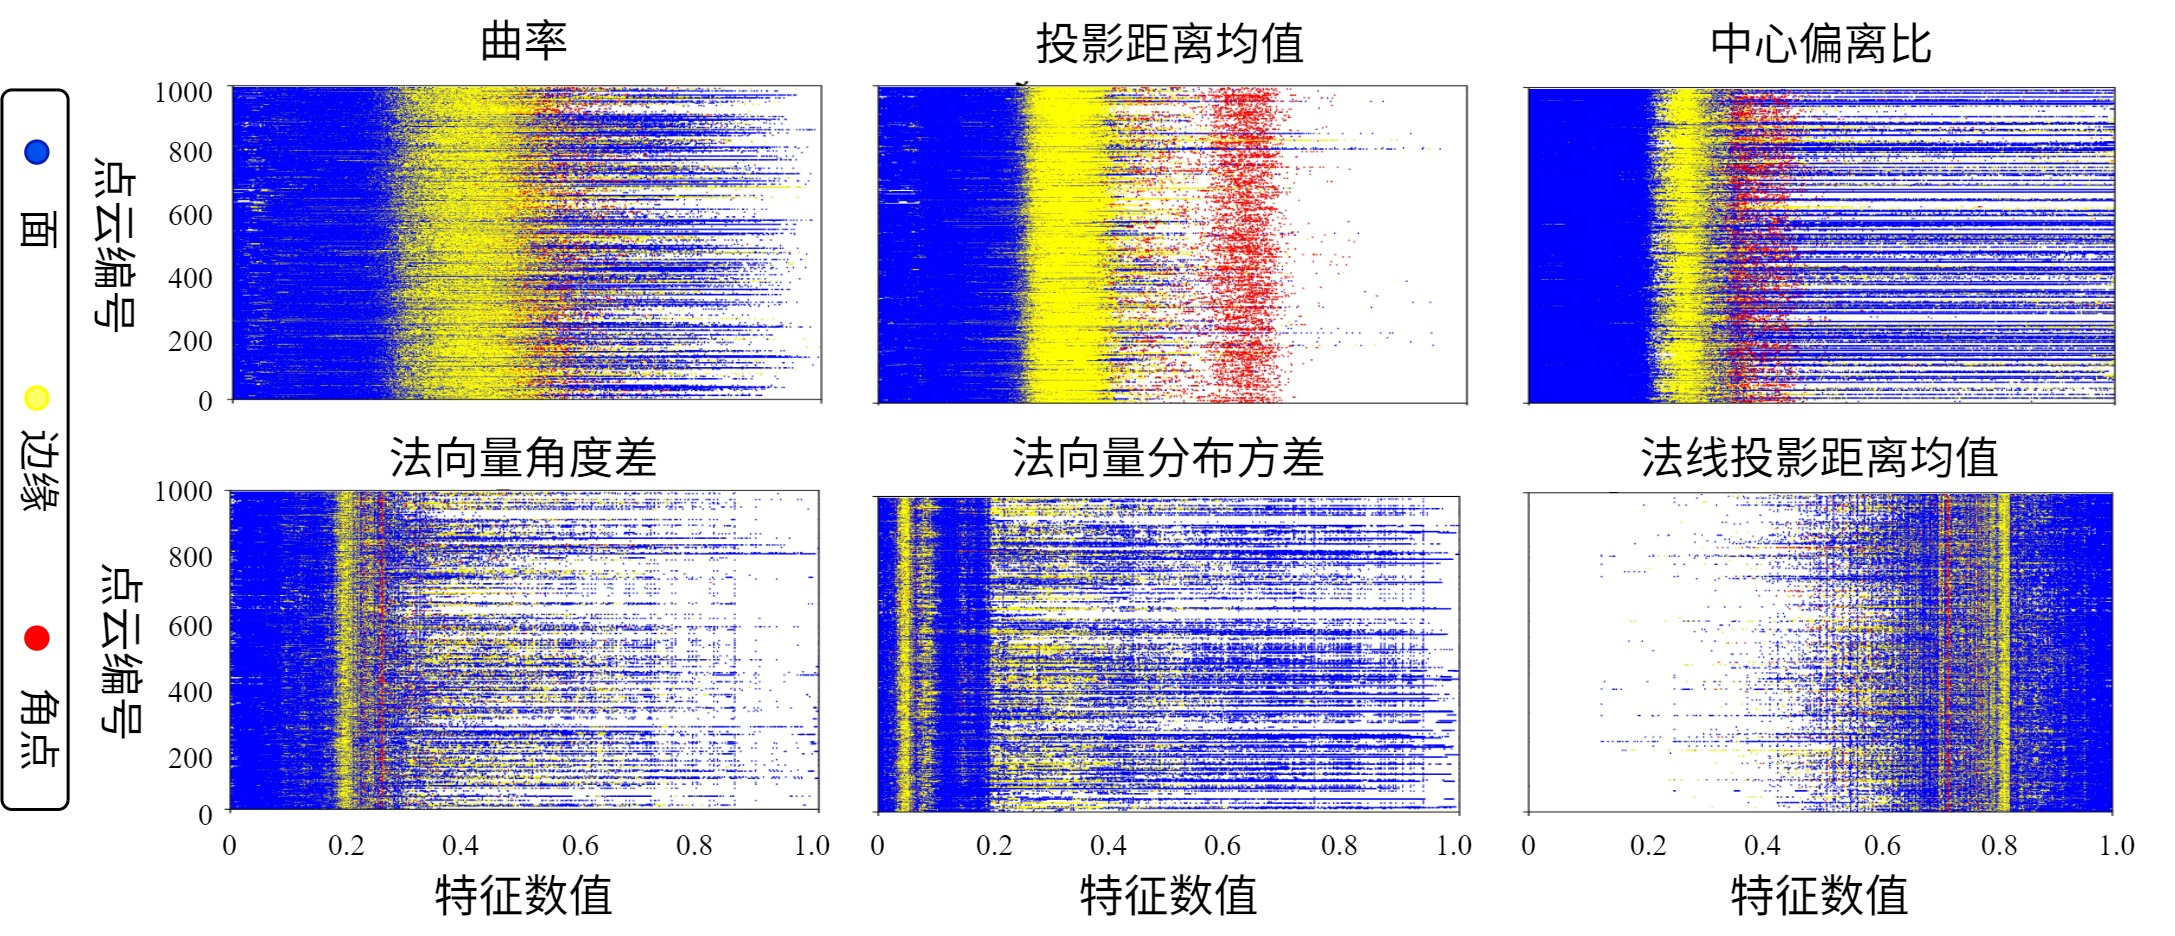
\includegraphics[width=1.0\textwidth]{NECDNet/feature_distribution.jpg}
    \bicaption{六个局部特征描述符在不同几何类别下的数值分布情况。}{Distribution of six local feature descriptors across different geometric categories.}
    \label{fig:feature_distribution}
\end{figure}


\section{\textrm{NECDNet} 网络架构设计}
% 阐述 MLP 基础的层次化网络结构。
% 多尺度特征矩阵的构建与输入。
% 分类器的设计与Dropout策略防止过拟合。
NECDNet 的网络架构设计基于多层感知机（Multi-Layer Perceptron, MLP）结构，旨在通过逐层融合多尺度局部特征矩阵，实现对点云中面点、边缘点和角点的高精度分类。该网络架构充分利用了前述计算的多尺度特征矩阵，结合深度学习的强大表达能力，有效捕捉点云局部几何结构的复杂关系。

图~\ref{fig:necdnet_architecture} 展示了 NECDNet 的具体网络结构。网络的输入为 $n$ 个查询点的多尺度特征矩阵 $\mathbf{X}_i^\text{c}$，其维度为 $n \times m \times 6$，其中 $m$ 为尺度数量（本文中取4）。网络整体可以分为两个本部分：多尺度特征融合及逐级分类。网络由多个全连接层（绿色）组成，每层后均采用 Leaky ReLU 激活函数（红色）以引入非线性变换，从而增强模型的表达能力。为了防止过拟合，网络中还引入了 Dropout 层（蓝色），在训练过程中随机丢弃部分神经元连接，提升模型的泛化能力。网络的输出为在，面、边缘、角点，三个类别上的分数，通过 Softmax 函数进行归一化获得，在三个类别中数值最大的类别即为最终的分类结果。
\begin{figure}[!htbp]
    \centering
    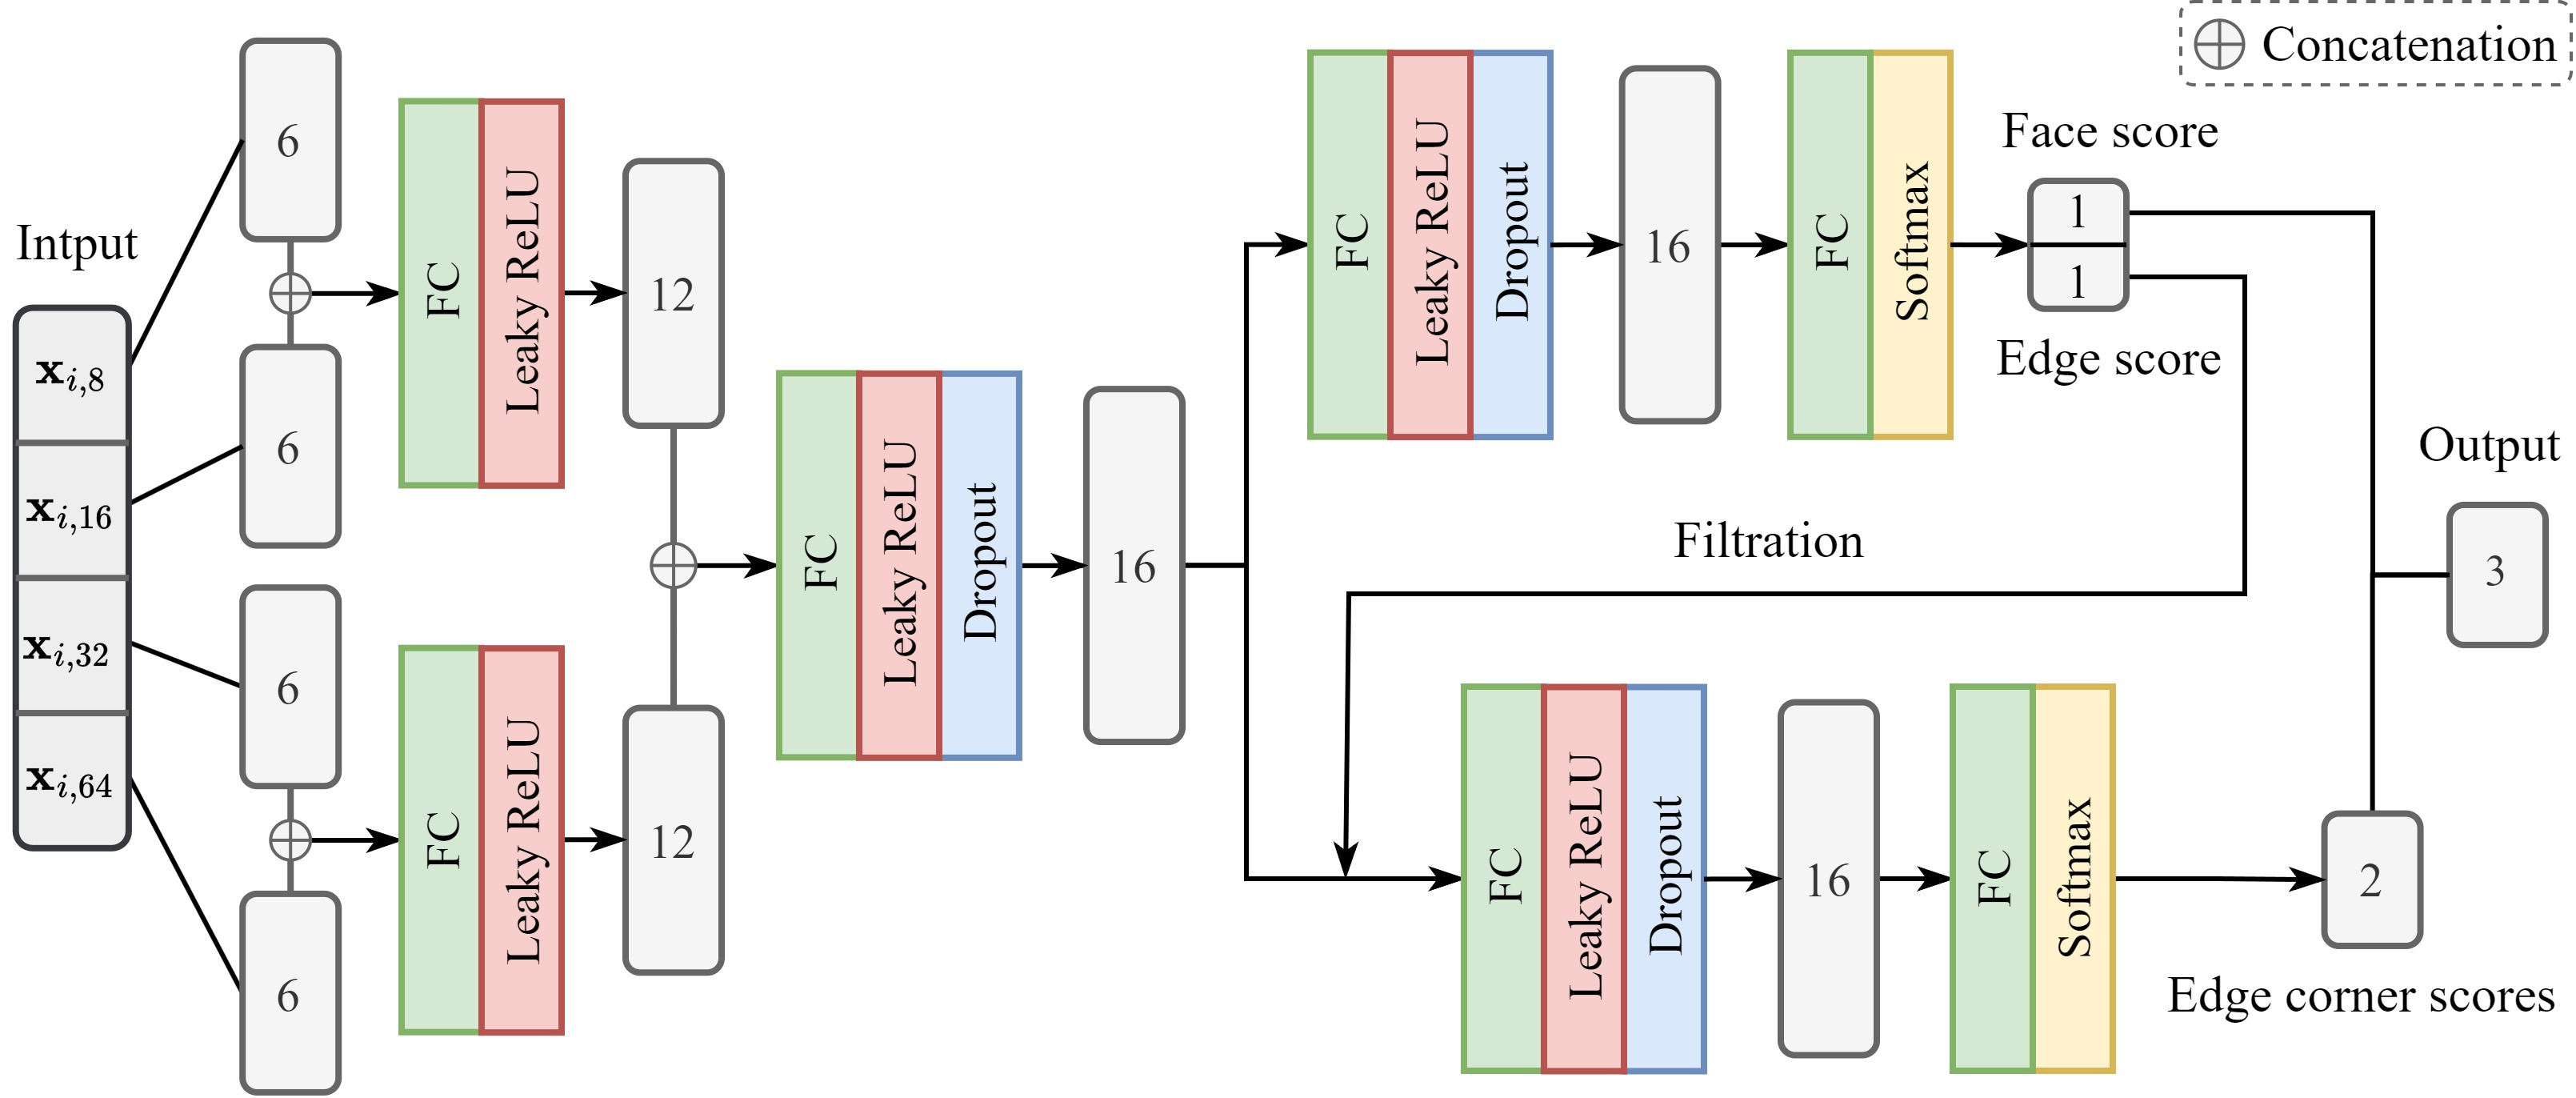
\includegraphics[width=1.0\textwidth]{NECDNet/necdnet_architecture.jpg}
    \bicaption{NECDNet 网络架构示意图。}{NECDNet network architecture diagram.}
    \label{fig:necdnet_architecture}
\end{figure}

\subsection{多尺度特征融合}
由于网络输入的数据是在多个邻域尺度下得到的，各个尺度下的特征矩阵包含了不同层次的局部几何信息。如果只是进行简单的拼接或平均处理，可能无法充分利用各尺度间的互补信息。因此，NECDNet 设计了逐层融合的机制，通过多层感知机对各尺度特征进行逐级整合，将特征的融合也作为网络的一部分进行学习。

具体而言，本文中输入的单个查询点的特征矩阵 $\mathbf{X}_i^\text{c}$ 包含四个尺度（$k=8,16,32,64$）下的六维特征。网络采用两两融合的方式，将输入的四个尺度的特征进行两两拼接（8和16，32和64）。随后，通过全连接层对拼接后的特征进行非线性变换和降维处理，得到融合后的特征向量，融合后的向量维度为 12。第二层对融合后的特征再次进行两两拼接，并通过全连接层进行进一步的融合和降维，最终得到一个 16 维的特征向量。其中降维到16是为了减轻后续的计算，使网络更加轻量化。此外，在进行非线性变换后，为了防止过拟合的现象，本文引入了Dropout层。最终的融合向量综合了不同尺度下的局部几何信息，为后续的分类任务提供了丰富的输入。

\subsection{逐级分类器}
特征融合后则进入逐级分类器部分。与特征融合类似，该部分也主要由全连接层组成，采用 Leaky ReLU 激活函数。但在具体结构上，逐级分类器部分使用分层设计，首先进行简单的分类任务（面、非面点），根据结果过滤非面点再进行更细粒度的分类（边缘、角点）。这种设计有助于简化分类任务，提高整体的分类准确率。

具体而言，首先让维度 16 的融合特征通过一个全连接层，输出维度为 8 的中间特征向量。随后，该中间特征向量通过另一个全连接层，输出维度为 2 的面、非面分类分数。根据该分数，本文采用阈值过滤的方式，将非面点送入下一级分类器进行边缘、角点的细粒度分类。下一级分类器同样由两个全连接层组成，首先将维度 8 的中间特征向量通过一个全连接层，输出维度为 4 的特征向量。随后，该特征向量通过另一个全连接层，输出维度为 2 的边缘、角点分类分数。最终，通过 Softmax 函数对三个分类分数进行归一化处理，得到每个类别的概率分布。
\subsection{损失函数}
点云中几何特征的分布存在不平衡现象，面点数量远多于边缘点和角点，特别是角点。为了应对类别不平衡问题，本文在训练过程中采用 Focal Loss 作为优化指标~\cite{}。该损失函数通过为不同类别分配不同的权重，增强对少数类别（边缘点和角点）的关注，从而提升模型在这些类别上的识别能力。

\subsection{评价指标}

\section{\textrm{ABC-Corner} 数据集构建}
\label{sec:dataset}
\subsection{数据集模型选取}
\subsection{初步标注}
\subsection{r}
% 介绍数据集来源（ABC dataset）及筛选标准。
% 详述标注流程（从CAD模型提取边缘 -> 几何规则提取粗角点 -> 人工精修）。
% 数据集的统计特性与类别不平衡处理（过采样策略）。

\section{本章小结}